\subsubsection{Fractionally Integrated GARCH} \label{link::figarch}
Пользуясь только что введенным методом дифференцирования рядов в фрактальном пространстве, анализируем поведение модели GARCH и переходим к так называемой FIGARCH. Первоначально имеем уравнение для GARCH (\myref{link::garch}). Однако теперь имеет смысл переписать его в более компактном виде:
\begin{equation}
	\sigma^2_t = \omega + \alpha_p(B)u^2_t + \beta_q(B)\sigma^2_t
\end{equation}
Где $\alpha_p(B)$ и $\beta_q(B)$ - полиномы соответствующих степеней от лагового оператора. Далее, пользуясь переобозначением вида $v_t = u_t^2 - \sigma^2_t = (\varepsilon^2_{t} - 1)\sigma^2_t: \varepsilon_{t} \sim N(0, 1)$, получаем эквивалентную запись \cite{tayefi2012overview}:
\begin{equation}
	\begin{split}
		u_t^2 & = \omega + \alpha_p(B)u_t^2 + \beta_q(B)u_t^2 - \beta_q(B)v_t + v_t\\
		\left[1 - \alpha_p(B) - \beta_q(B)\right] u_t^2 & = \omega + \left[1 - \beta_q(B)\right]v_t
	\end{split}
\end{equation}
Подобная запись уже очень похода на ARMA, однако определяется данная модель иначе, а точнее - ARMA$(m, q): m = \max(p, q), v_t = u_t^2 - \sigma^2_t$. Интересно, что процесс $v_t$ интерпретируется как шоки для условной дисперсии, так как $\E(v_t) = \E(u_t^2 - \sigma^2_t) = \E(u_t^2) - \E(\sigma^2_t) = 0$. Следовательно интегрированный GARCH процесс записывается как:
\begin{equation} \label{link::approx_figarch}
	\left[1 - \alpha_p(B) - \beta_q(B)\right] (1 - B) u_t^2 = \omega + \left[1 - \beta_q(B)\right]v_t
\end{equation}
Финальным штрихом при переходе от GARCH к FIGARCH является замена 1-й разности в $(1 - B)$ на дробно интегрированную, где $(1 - B)^d: d \in (0, 1)$. В итоге выражение (\ref{link::approx_figarch}) становится:
\begin{equation} \label{link::approx_figarch}
	\left[1 - \alpha_p(B) - \beta_q(B)\right] (1 - B)^d u_t^2 = \omega + \left[1 - \beta_q(B)\right]v_t
\end{equation}
Таким образом, получаем модель, способную описывать более сложные временные колебания в данных, в том числе и финансовых, по сравнению с другими GARCH-подобными моделями \cite{davidson2004moment}. Также отмечаем, что $(1 - B)^d$ можно расписать не только так, как было сделано для модели ARFIMA (\myref{link::fractual_difference}), но и в виде:
\begin{equation}
	(1 - B)^d = \sum_{k = 0}^\infty \frac{\Gamma(k - d)}{\Gamma(k + 1)\Gamma(-d)}B^k
\end{equation}
Для оценки параметров данной модели используется Maximum Likelihood Estimation (Метод Максимального Правдоподобия), однако, исходя из реальных исследований, имеем, что предположение о нормальном распределение остатков в случае с методом MLE (ММП) приводит к более плохому результату, чем применение устойчивого метода quasi-MLE, описанного в \cite{weiss1986asymptotic}. Аналогично всему предыдущему проводим эксперимент, основываясь на доходностях цены открытия акций Apple. В итоге получаем сводную таблицу моделей вида:

\begin{table}[H]
	\centering
	\begin{tabular}{c|cccc}
		\toprule
		& $(0, d, 0)$ & $(1, d, 0)$ & $(0, d, 1)$ & $(1, d, 1)$\\
		\midrule[0.02cm]
		$\mu$ & \setval{0.099}{***}{0.022} & \setval{0.099}{***}{0.022} & \setval{0.106}{***}{0.013} & \setval{0.105}{***}{0.027}\\[0.2cm]
		$\omega$ & \setval{1.108}{***}{0.107} & \setval{1.108}{***}{0.126} & \setval{0.589}{***}{0.090} & \setval{0.308}{***}{0.088}\\[0.2cm]
		$\alpha_1$ & - &  \setval{0.000}{}{0.025} & - & \setval{0.273}{***}{0.082}\\[0.2cm]
		$d$ & \setval{0.212}{***}{0.010} & \setval{0.212}{***}{0.010} & \setval{0.290}{***}{0.020} & \setval{0.329}{***}{0.026}\\[0.2cm]
		$\beta_1$ & - & - & \setval{0.190}{***}{0.027} & \setval{0.492}{***}{0.085}\\[0.2cm]
		\midrule[0.02cm]
		$\nu$ &  \setval{1.199}{***}{0.027} & \setval{1.199}{***}{0.027} & \setval{1.206}{***}{0.026} & \setval{1.205}{***}{0.027}\\[0.05cm]
		BIC & $48'832$ & $48'841$ & $48'774$ & $48'772$\\[0.05cm]
		$n$ & $10'560$ & $10'560$ & $10'560$ & $10'560$\\
		\midrule[0.02cm]
		Note: & \multicolumn{4}{r}{*$p < 0.1$, **$p < 0.05$, ***$p < 0.01$}\\
	\end{tabular}
	\caption{Сводная таблица моделей FIGARCH}
\end{table}

\noindent Замечаем, что в каждой модели параметр $d$ значим на $1\%$-ом уровне и, если вычислять значение экспоненты Херста, то в каждой случае получаем персистентный процесс. Однако как и в предыдущих моделях, информационный критерий BIC позволяет выявить лучшую с точки зрения описания данных - FIGARCH$(1, 0.329, 1)$, что даже меньше, чем в случае с моделью GARCH$(1, 1)$ (\myref{link::garchs}), где BIC = $50'056$. То есть полученная модель еще качественнее описывает данные. Однако также в сводной таблице имеется некоторый показатель $\nu$, относящийся к обобщенному нормальному распределению, плотность которого в общем виде задается формулой:
\begin{equation}
	p_\xi(x) = \frac{\nu}{2 \sigma \Gamma(1 / \nu)} \exp \left(-\left\{|x - \mu|/\sigma\right\}^\nu \right)
\end{equation}
Где $\sigma$ - фактор сжатия/разжатия, $\mu$ - расположения распределения относительно среднего значения, а $\nu$ - это некоторый гиперпараметр формы. Графически Generalized Normal Distribution (GND) в стандартном случае, то есть при $\mu = 0$ и $\sigma = 1$, имеет вид:
\begin{figure}[H]
	\centering
	\begin{tikzpicture}
		\begin{axis}[
			grid = both,
			legend pos = north west,
			minor tick num = 1,
			major grid style = {lightgray},
			minor grid style = {lightgray!25},
			title= {$f(x, \nu) = \frac{\nu}{2 \Gamma(1 / \nu)} \exp \left(-|x|^\nu \right)$},
			width = \textwidth,
			height = 0.5 \textwidth,
			xmin=-5, xmax=5,
			ymin=0, ymax=0.6,
			line width=0.3mm
			]
			\addplot table [
			x=x, 
			y=y_0_5, 
			col sep=comma,
			mark={},
			] {./source/source_csv/Illustration data/figarch/gennormal_dist.csv};
			%\legend{AAPL 2021};
			
			\addplot table [
			x=x, 
			y=y_1_0, 
			col sep=comma,
			mark={},
			] {./source/source_csv/Illustration data/figarch/gennormal_dist.csv};
			%\legend{EWMA $\beta = 0.1$};
			
			\addplot table [
			x=x, 
			y=y_1_5, 
			col sep=comma,
			mark={},
			] {./source/source_csv/Illustration data/figarch/gennormal_dist.csv};
			%\legend{EWMA $\beta = 0.1$};
			
			\addplot table [
			x=x, 
			y=y_2_0, 
			col sep=comma,
			mark={},
			] {./source/source_csv/Illustration data/figarch/gennormal_dist.csv};
			%\legend{EWMA $\beta = 0.3$};
			
			\addplot table [
			x=x, 
			y=y_2_5, 
			col sep=comma,
			mark={},
			] {./source/source_csv/Illustration data/figarch/gennormal_dist.csv};
			%\legend{EWMA $\beta = 0.5$};
			
			\addplot table [
			x=x, 
			y=y_3_0, 
			col sep=comma,
			mark={},
			] {./source/source_csv/Illustration data/figarch/gennormal_dist.csv};
			
			\addplot table [
			x=x, 
			y=y_3_5, 
			col sep=comma,
			mark={},
			] {./source/source_csv/Illustration data/figarch/gennormal_dist.csv};
			
			\addplot table [
			x=x, 
			y=y_4_0, 
			col sep=comma,
			mark={},
			] {./source/source_csv/Illustration data/figarch/gennormal_dist.csv};
			
			\addplot table [
			x=x, 
			y=y_8_0, 
			col sep=comma,
			mark={},
			] {./source/source_csv/Illustration data/figarch/gennormal_dist.csv};
			
			\legend{$\nu = 0.5$, $\nu = 1.0$, $\nu = 1.5$, $\nu = 2.0$, $\nu = 2.5$, $\nu = 3.0$, $\nu = 3.5$, $\nu = 4.0$, $\nu = 8.0$};
		\end{axis}
	\end{tikzpicture}
	\caption{GND$(\mu = 0, \sigma = 1)$}
\end{figure}
\noindent Подобное необычное распределение использовано для наиболее точного описания данных посредством введения предпосылки о распределении остатков модели. Теперь смотрим на построенные ею (моделью) прогнозные значения волатильности и показателя доходности.
\begin{figure}[H]
	\centering
	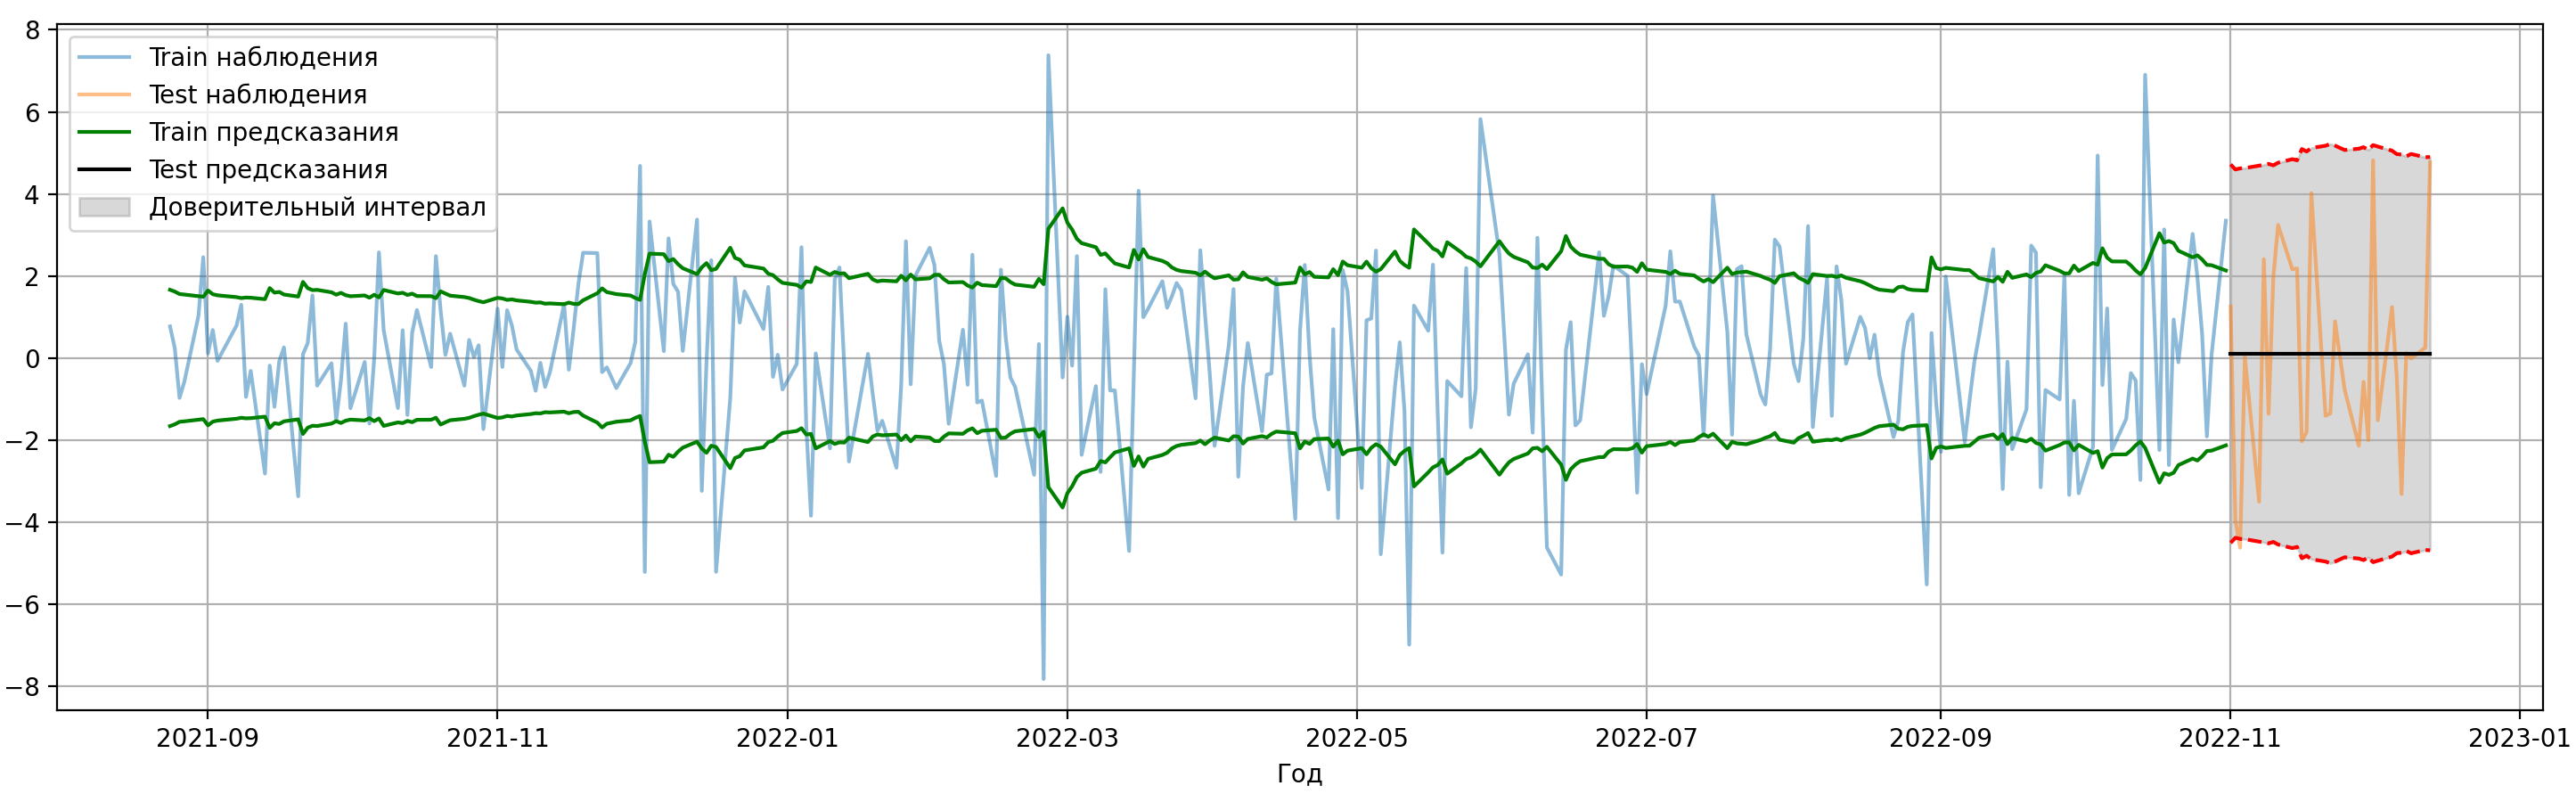
\includegraphics[width=17cm]{figarch/predicton.png}
	\caption{Предсказания доходности (в \%) и волатильности моделью FIGARCH$(1, 0.329, 1)$ на 30 рабочих дней биржи}
\end{figure}
\noindent И далее смотрим на прогнозирование показателя условной дисперсии:
\begin{figure}[H]
	\centering
	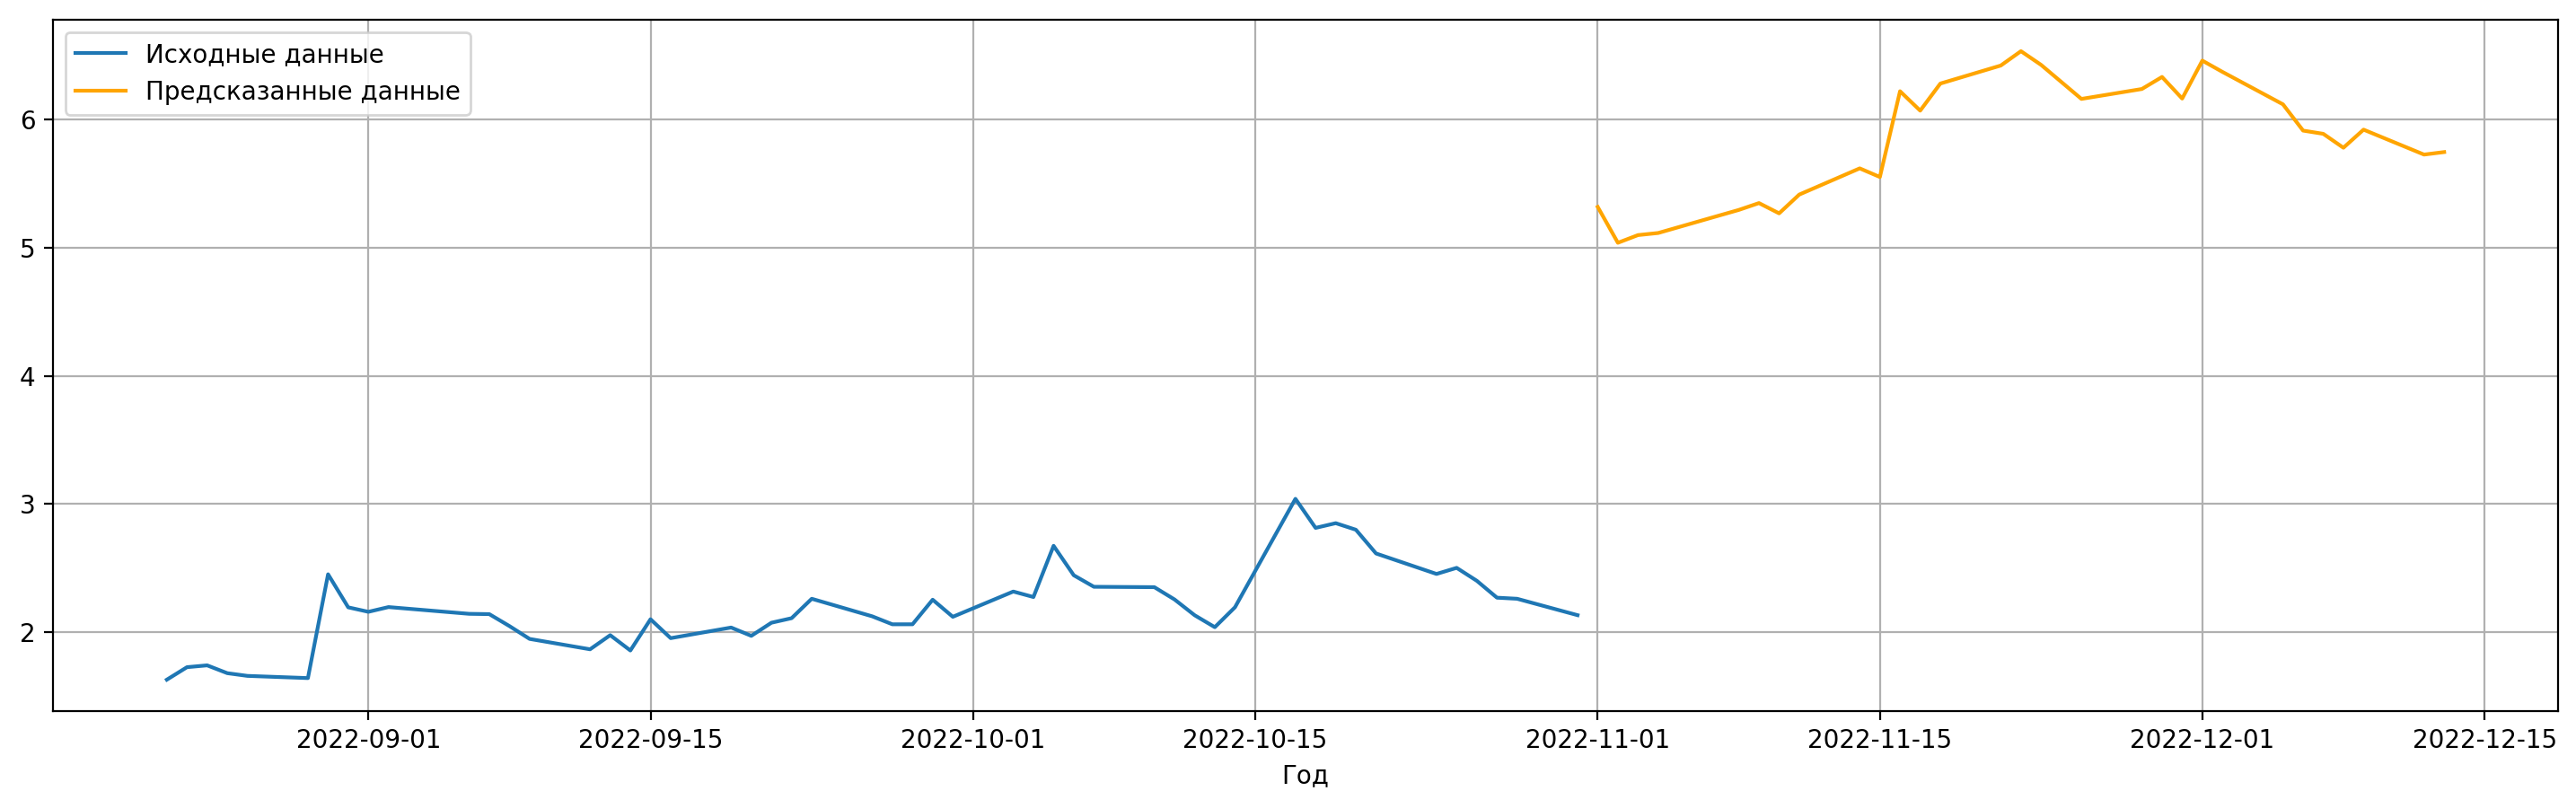
\includegraphics[width=17cm]{figarch/cond_heter_forecast.png}
	\caption{Предсказание условной гетероскедастичности моделю FIGARCH$(1, 0.329, 1)$}
\end{figure}
\noindent Для интереса и сравнения с поведением GARCH, основываясь на графике ниже, описание исходного набора данных имеет более <<ребристый>> вид, что говорит о большей чувствительности модели к изменению поведения условной гетероскедастичности:
\begin{figure}[H]
	\centering
	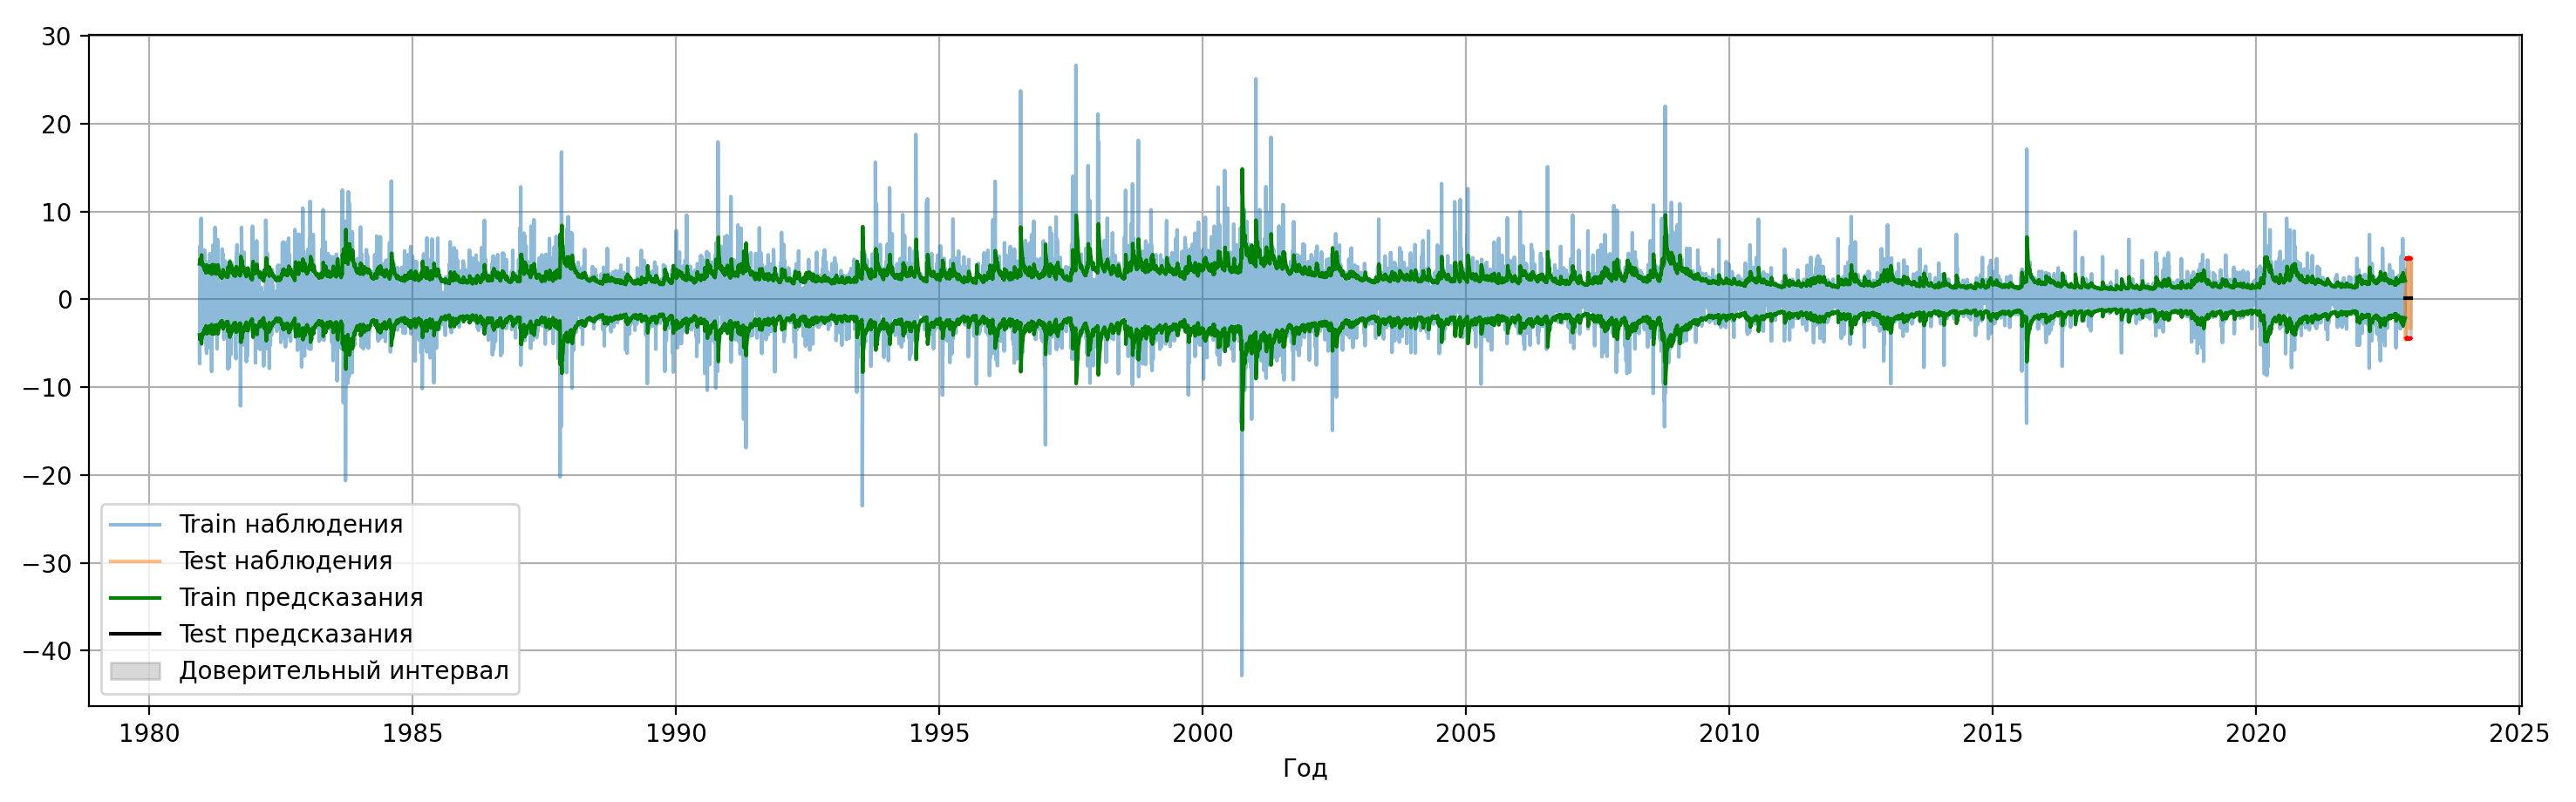
\includegraphics[width=17cm]{figarch/predicton_long.png}
	\caption{Предсказание условной гетероскедастичности моделю FIGARCH$(1, 0.329, 1)$ для всего набора данных}
\end{figure}

\noindent В итоге получаем, что модель FIGARCH лучше описывает условную гетероскедастичность, чем модель GARCH. Это не делает GARCH менее применимым, однако, исходя из статистических соображений только что проведенного эксперимента, предполагаем, что FIGARCH позволяет достичь более качественного результата в описании данных для рынка, на котором выполняются условия фрактальности \cite{fractal_market}. FIGARCH включается в итоговую таблицу.